%%% LaTeX Template: Article/Thesis/etc. with colored headings and special fonts
%%%
%%% Source: http://www.howtotex.com/
%%% Feel free to distribute this template, but please keep to referal to http://www.howtotex.com/ here.
%%% February 2011
%%%
%%% Modified October 2015 by CDM

%%%  Preamble
\documentclass[11pt,letterpaper]{article}
\usepackage[margin=1.0in]{geometry}
\usepackage[T1]{fontenc}
\usepackage[bitstream-charter]{mathdesign}
\usepackage[latin1]{inputenc}					
\usepackage{amsmath}						
\usepackage{xcolor}
\usepackage{cite}
\usepackage{hyphenat}
\usepackage{graphicx}
\usepackage{float}
\usepackage{subfigure}
\usepackage{sectsty}
\usepackage[compact]{titlesec} 
\usepackage[tablegrid]{vhistory}
\allsectionsfont{\color{accentcolor}\scshape\selectfont}

%%% Definitions
\definecolor{accentcolor}{rgb}{0.0,0.0,0.5} 
\newcommand{\teamname}{Boring Torvalds}
\newcommand{\productname}{Smart Mirror}
\newcommand{\coursename}{CSE 4316: Senior Design I}
\newcommand{\semester}{Fall 2016}
\newcommand{\docname}{Project Charter}
\newcommand{\department}{Department of Computer Science \& Engineering}
\newcommand{\university}{The University of Texas at Arlington}
\newcommand{\authors}{William G. Hilliard \\ Dylan Ebert \\ Kevin Frances \\ Joel Melendez \\ Nhat Dao}

%%% Headers and footers
\usepackage{fancyhdr}
	\pagestyle{fancy}						% Enabling the custom headers/footers
\usepackage{lastpage}	
	% Header (empty)
	\lhead{}
	\chead{}
	\rhead{}
	% Footer
	\lfoot{\footnotesize \teamname \ - \semester}
	\cfoot{}
	\rfoot{\footnotesize page \thepage\ of \pageref{LastPage}}	% "Page 1 of 2"
	\renewcommand{\headrulewidth}{0.0pt}
	\renewcommand{\footrulewidth}{0.4pt}

%%% Change the abstract environment
\usepackage[runin]{abstract}			% runin option for a run-in title
%\setlength\absleftindent{30pt}			% left margin
%\setlength\absrightindent{30pt}		% right margin
\abslabeldelim{\quad}	
\setlength{\abstitleskip}{-10pt}
\renewcommand{\abstractname}{}
\renewcommand{\abstracttextfont}{\color{accentcolor} \small \slshape}	% slanted text

%%% Start of the document
\begin{document}

%%% Cover sheet
{\centering \huge \color{accentcolor} \sc \textbf{\department \\ \university} \par}
\vspace{1 in}
{\centering \huge \color{accentcolor} \sc \textbf{\docname \\ \coursename \\ \semester} \par}
\vspace{0.5 in}
\begin{figure}[h!]
	\centering
   	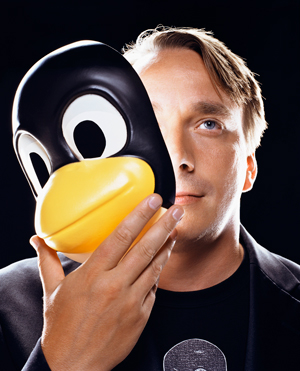
\includegraphics[width=0.60\textwidth]{images/boring_torvalds}
\end{figure}
\vspace{0.5 in}
{\centering \huge \color{accentcolor} \sc \textbf{\teamname \\ \productname} \par}
\vspace{0.5 in}
{\centering \large \sc \textbf{\authors} \par}
\newpage


%\vspace{1 in}
%\centerline{January 13th, 2012}
%\newpage

%%% Revision History
\begin{versionhistory}
  	\vhEntry{0.1}{10.04.2016}{KF, WH, DE, JM, ND}{document creation}
\end{versionhistory}
\newpage

%%% Table of contents
\tableofcontents
\newpage

%%% List of figures and tables (optional)
\listoffigures
%\listoftables
\newpage

%%% Agile project charter sections
\section{Vision}
Previous studies have shown that it is common for a typical morning to consist of t	wo tasks: looking in the mirror, and looking at one's phone. Our vision involves improved convenience and efficiency for users through the combination of these tasks by allowing the user to view life updates otherwise seen on the phone, in the mirror.
\section{Mission}
Our mission is to develop a smart mirror that displays pertinent information to users. The mirror will recognize the user through facial recognition techinques in order to display their desired information. It shall be customizable machine learning and interface with the user via multiple methods.
\section{Success Criteria}
-Camera with facial recognition to recognize the user\newline
-Display weather information\newline
-Display personal notifications from mail, social networks, etc.\newline
-Voice-based interaction\newline
-REST-based interaction\newline
-Video demo
\newpage

%%% Remaining project charter sections
\section{Background}
The project was proposed by the client in order to automate routine morning tasks. If successful, this project will stream line "morning rituals" and enhance the user's quality of life.
\section{Related Work}
The concept of a smart mirror exists as personal projects by others, but we intend to improve upon the concept. The difference with our project is the presence of facial recognition, machine-learning preferences, and tentative additional features to be added later.\newline
https://www.youtube.com/watch?v=sh2EJzplkpM
\section{System Overview}
Our system will include a two way mirror with an LCD screen, computer, camera, and speaker behind it. The LCD screen will show applications that are programmed on the computer. The user will be able to interact with the applications via voice and facial recognition. The user will also be able to customize the display remotely.
\section{Roles \& Responsibilities}
Some general stated relevant areas of expertise are as follows:\newline
-Dylan: Facial recognition, GUI\newline
-Joel: Hardware Assembly, Android-App interface\newline
-Nhat: Machine Learning / Logic / Systems \newline
-Grayson: RESTful Server Implimentation / Systems \newline
-Kevin: Mobile app
\section{Facilities \& Equipment}
Facilities we will be using will be the Senior Design Lab and Senior Design Classrooms. We will use the Senior Design Lab for storing our materials and constructing our product. We will be using the Senior Design Classrooms for meeting and working on other parts of the project.
Equipment we will use includes various modules. Our tentative list of equipment is as follows:\newline
-Two-way glass material from twowaymirrors.com, for the actual mirror\newline
-LED display to go behind the mirror and display information\newline
-RGBD camera for the facial recognition\newline
-Intel NUC for the backend computer\newline
-Amazon Echo (Alexa) for voice interaction
\section{Cost Proposal}
Due to agile nature of the project, a full feature list has yet to be completed. However, the first set of usercases will provide a base cost that may fluctuate depending on donations and discounts.

\subsection{Preliminary Budget}
\$400 for Display\newline
\$209/free for Mirror\newline
\$629 for Intel NUC\newline

\subsection{Current \& Pending Support}
The current funds for this project have come from department sponsorship which total to 800. We also had parts donated to us by Reflective Security LLc and knowledge donated by Oaklabs. We are also attempting to get the Intel NUC at a reduced price.
\section{Documentation \& Reporting}


\subsection{Project Charter}
This document is the Project Charter. It is a high-level plan for the project and our first task.

\subsection{Product Backlog}
The Product Backlog will manifest itself in the form of a column of a Trello Task Board. By utilizing Trello's online organization features, we will be able to dynamically adjust the backlog, assign proirity to features, assign work, document progress, and maintain a comprehensive work log.

\subsection{Sprint Planning}
We will prioritize the immediate goals first, then work on additional functionalities. We will track the progress of these goals via a repository wiki in project's Github. Kevin will be Scrum Master. 

\subsubsection{Sprint Goal}
The team will vote on each sprint goal. Any disputes will be mediated by the professor.

\subsubsection{Sprint Backlog}
Scrum Master (Kevin) will pull items from product backlog. Team will vote on size of sprint backlog. We will still pull lower dependencies in backlog.

\subsubsection{Task Breakdown}
We will agree upon task assignment for each sprint, based on volunteering. The task division will be based on roles.
Their areas of expertise will be considered in task assignment.

\subsection{Sprint Burndown Charts}
The team shall evaluate the feature backlog and utilize the Sprint Burndown Charts in order to establish a priority queue. The approximate time estimates shall be measured in terms of a sprint length and the approximate effort estimates shall be measured in terms of difficulty with respect to the first completed feature.

% \begin{figure}[h!]
%     \centering
%     
\includegraphics[width=0.5\textwidth]{images/test_image}
%     \caption{Example sprint burndown chart}
% \end{figure}

\subsection{Sprint Retrospective}
We will discuss what went well with each Sprint and what were areas that needed improvement. At the end of each cycle, we will discuss how to do things differently to make the next cycle run smoother.  

\subsection{Individual Status Reports}
Individual status reports will be given verbally at each scrum meeting. Those who can't attend will be required to submit a written update.

\subsection{Engineering Notebooks}
Team will sign on each others.

\subsection{Closeout Materials}
Our closeout materials include a minimum of the following:\newline
-Working Smart Mirror system\newline
-Video demo of the working system\newline
-Some form of documentation\newline

\subsubsection{Web Page}
We will have a web page hosted by Github to showcase our project.

\subsubsection{Source Code}
Source code and its versions are managed with git. 

\subsubsection{Source Code Documentation}
All source code shall be uploaded to GitHub / BitBucket in a repository in order to maintain version control and integrity. Clone requests shall be granted for all team members but restricted for all else until a designated "turnover" point.

\subsubsection{Hardware Schematics}
   	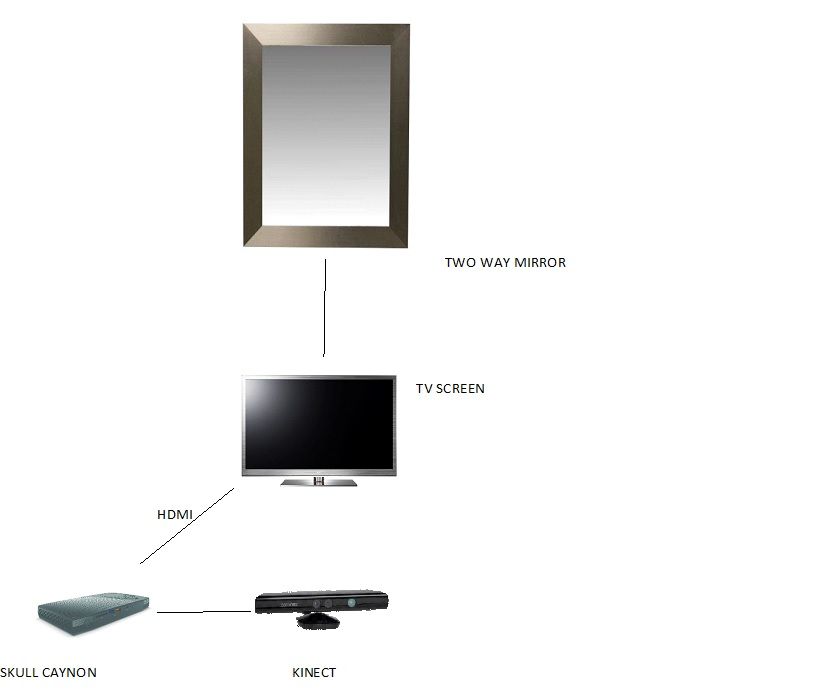
\includegraphics[width=0.90\textwidth]{images/Schematic}

\subsubsection{CAD files}
We will use Github to host our git repositories.

\subsubsection{Installation Scripts}
With the mirror as the hypothetical product, software would be preinstalled and ready for use out-of-the-box. As of our high-level definition, no installation scripts are defined. Live updates, modability, and manual installation will have to be of consideration later in the project, depending on the progress of crucial features.

\subsubsection{User Manual}
The user manual shall be comprised of Markdown text documents which shall be stored in the respective GitHub / BitBucket repository in order to maintain version control and integrity.
\newpage

%%% References
\bibliographystyle{plain}
\bibliographystyle{reference/IEEEtran_custom}
\bibliography{reference/refs}{}

\end{document}